\chapter{Communication Volume Calculation} \label{cv_calculation}
This chapter extends the discussion from Section~\ref{sec:greedy_refinement} of Chapter~\ref{chap:multilevel-kway}, where we showed how the change in the objective function's value (the gain) is computed for the edge-cut objective function. Here, we derive the analogous gain computations for two objective functions based on communication volume: the total communication volume objective function (VOL) and our partition-aware communication volume objective function NVOL. The next chapter then shows how these gain calculations are used inside the greedy refinement algorithm.

The chapter is organized into four sections. The first introduces the basic definitions needed to understand communication volume operations. The second describes the gain calculation for VOL, which is more representative of actual communication cost than edge-cut, although it does not necessarily yield a well-balanced result. We treat VOL first because it is the standard approach used by partitioners such as METIS.

The third section presents our novel gain calculation, used by NVOL, which provides finer information about how the volume of each individual partition is affected by a move. Here each vertex has a table representing the partition-specific gain of all possible moves. The section ends with an algorithm that ties the calculation together. The fourth and final section works through a few concrete examples to give the reader a clearer picture of how everything fits together.

\begin{table}[h]
%	\centering
	\label{tab:notation}
	\begin{tabular}{cl}
		\toprule
		\textbf{Symbol} & \textbf{Description} \\
		\midrule
		$G$          & The graph \\
		$V$			& Set of all vertices in the graph\\
		$E$			& Set of all edges in the graph\\
		$V_b$		& Set of all boundary vertices in the graph\\
		$V^{\mathrm{adj}}_i$ & Set of all vertices incident to vertex $i$\\
		$N_i$        & Set of neighboring partitions of vertex $i$ \\
		$N_{iv}$      & Set of partitions neighboring both vertex $i$ and  vertex $v$\\
		$N_{i-v}$    & Set of partitions only neighboring vertex $i$ and not vertex $v$\\
		$w(i)$		& Vertex weight of vertex $i$\\
		$P[i]$		& Partition of vertex $i$\\
		$PV[a]$		& Outgoing communication volume of partition $a$\\
		$C_i[n]$	& Number of edges a vertex $i$ has to a partition $n$\\
		$G_i$		& Gain vector of a vertex $i$\\
		$SG_i$		& Gain table of a vertex $i$\\	
		\bottomrule
	\end{tabular}
	\caption{Notation used in Chapter~\ref{cv_calculation}.}
\end{table}
\section{Basic definitions}
To facilitate understanding of how gain calculation works, we begin by introducing a formal definition of communication volume. Let $G = (V, E)$ be a graph, and let $P$ be the partition vector, where $P[v]$ is the partition a vertex \textit{v} is assigned to. A vertex $u$ is defined as a neighbor of $v$ if there exists an edge $\{u,v\} \in E$. Any vertex adjacent to at least one vertex belonging to a different partition is said to lie on the boundary. We denote the set of all boundary vertices by $V_b \subseteq V$. Formally, $v \in V_b$ if there exists at least one neighbor $u \in V$ such that $\{v,u\} \in E$ and $P[v] \neq P[u]$.

For each boundary vertex $v \in V_b$, let $N_v$ denote the set of distinct partitions (excluding $P[v]$) to which its neighboring vertices belong. The number of partitions contained in $N_v$, defined as $\lvert N_v \rvert$, is the outgoing communication volume of vertex $v$. Note that the number of edges incident to $v$ is not directly relevant for this measure, only the number of distinct neighboring partitions. In Figure~\ref{1}, vertex $A$ has an outgoing communication volume of 2, as it is connected to vertices in two distinct partitions. In contrast, Figure~\ref{2} illustrates a case where vertex $A$ has two edges, both connecting to vertices within the same partition. Consequently, the outgoing communication volume of vertex $A$ is 1, since only a single neighboring partition is involved.

\begin{figure}[H]
	\centering
	\begin{minipage}[b]{.4\textwidth}
		\centering
		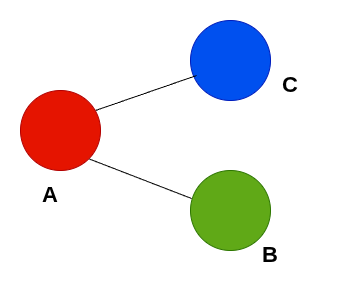
\includegraphics[width=.7\linewidth]{pictures/node_volume_2}
		\caption{Vertex $A$ has an outgoing communication volume of 2. Each color represents a partition.}
		\label{1}
	\end{minipage}\qquad
	\begin{minipage}[b]{.4\textwidth}
		\centering
		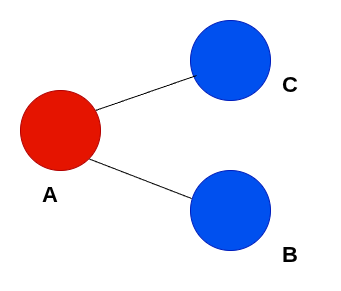
\includegraphics[width=.7\linewidth]{pictures/node_volume_1}
		\caption{Vertex $A$ has an outgoing communication volume of 1. Each color represents a partition.}
		\label{2}
	\end{minipage}
\end{figure}

The total communication volume of the partitioned graph is obtained by summing the outgoing volumes over all boundary vertices:
\begin{equation} \label{total_volume}
	\mathrm{total~volume} = \sum_{v \in V_b} \left| N_v \right|w(v)
\end{equation}
Here, $w(v)$ denotes the weight associated with vertex $v$, which scales its contribution to the outgoing communication volume. Even if the original graph has unit vertex weights, vertices acquire non-unit weights during coarsening as a result of vertex aggregation, and these weights persist during uncoarsening (see Section~\ref{sec:uncoarsening}). In Figure~\ref{tot_vol_example}, all vertices are assumed to have unit weight. The boundary set is $V_b = \{A, B, C, D, E\}$. Note that vertex \textit{F} is not part of this set, as it has no edges connecting to vertices in other partitions.

Applying Equation~\ref{total_volume}, we compute the total communication volume  by summing the contributions of all vertices in the boundary set. Vertices \textit{A}, \textit{C}, and \textit{D} each contribute a volume of 2, while vertices \textit{B} and \textit{E} each contribute a volume of 1. This results in a total communication volume of 8.
\begin{figure}[H]
	\centering
	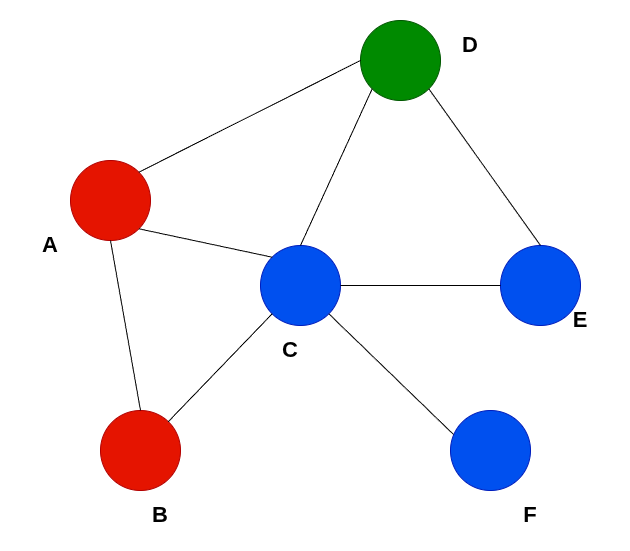
\includegraphics[width=.35\linewidth]{pictures/tot_vol_example}
	\caption{The total communication volume is 8.}
	\label{tot_vol_example}
\end{figure}

\section{VOL gain calculation} \label{METIS gain calculation}
This section describes how the gain resulting from a vertex move is computed for VOL. All definitions are deduced from METIS's implementation, but the approach is standard and applies to any implementation of a total communication volume objective function. The gain for VOL represents the change in total communication volume resulting from relocating a vertex to a new partition: a positive gain indicates a reduction, a negative gain an increase. 

Since communication only arises when an edge connects two vertices belonging to different partitions, a vertex move can only affect the communication volume of its neighboring partitions. For each boundary vertex $i \in V_b$, a partitioner needs to examine all its adjacent vertices $v \in V^{\mathrm{adj}}_i$, where $V^{\mathrm{adj}}_i \subseteq V$ denotes the set of vertices adjacent to $i$. When considering moving a boundary vertex \textit{i}, the gain calculation depends on the relationship that \textit{i} and each of its neighboring vertices have with other partitions. The effect on volume depends on which partitions they share. To support our calculations later, we define, for every vertex \textit{i} and every neighboring vertex \textit{v}
\begin{equation}
	N_{i-v} = N_i \setminus (N_v \cup P[v])
	\quad \text{and} \quad
	N_{iv} = (N_i \cap N_v) \cup P[v]
\end{equation}
representing partitions exclusive to $i$ and partitions shared by $i$ and $v$, respectively. Notice how both sets are subsets of $N_i = N_{i-v} \cup N_{iv}$. Recall that by definition $N_v$ excludes $v$'s own partition $P[v]$. To correctly identify shared partitions, $P[v]$ must therefore be added to $N_{iv}$ and removed from $N_{i-v}$. 

As a concrete example, consider Figure~\ref{tot_vol_example} and suppose the candidate vertex is~$A$, with neighbor~$B$ under consideration. Here, $N_A = \{\mathrm{blue}, \mathrm{green}\}$, while $N_B = \{\mathrm{blue}\}$. Consequently, $N_{A-B} = \{\mathrm{green}\}$, since green is the only partition connected to~$A$ but not to~$B$, whereas $N_{AB} = \{\mathrm{blue}\}$ as both vertices have at least one edge to the blue partition. Keeping \textit{A} as the candidate vertex, consider now neighbor~$C$ with $N_C = \{\mathrm{red}, \mathrm{green}\}$. \textit{A} and \textit{C} have access to the same partitions, meaning that $N_{A-C} = \emptyset$ and $N_{AC} = \{\mathrm{blue}, \mathrm{green}\}$. This example highlights the need for adding $P[C]$ to the sets. The sets would have been $N_{A-C} = \{\mathrm{blue}\}$, $N_{AC} = \{\mathrm{green}\}$ if we had not accounted for $P[C]$. However, from Figure~\ref{tot_vol_example} we can see that the blue partition is shared and not unique to \textit{A}.

Since communication volume is a more complex metric to calculate, and cannot be evaluated on-the-fly like edge-cut, we need to expand our definitions. We define a gain vector $G_i$ with a number of elements equal to the number of partitions, initialized to 0, where $G_i[a]$ represents the total gain obtained by moving vertex $i$ to partition $a$. To determine which contributions to apply to $G_i$, we will also need to count edges between a vertex and a specific partition. Let $C_i[a]$ denote the number of edges connecting $i$ to partition $a$. In Figure~\ref{tot_vol_example}, for example, $C_A[\mathrm{blue}] = 1$, as \textit{A} has only one edge connected to the blue partition, while $C_D[\mathrm{blue}] = 2$, as \textit{D} has two edges connected to the blue partition. 

For a candidate vertex \textit{i} being considered for a move, the gain resulting from moving $i$ to a partition is evaluated by iterating over all neighboring vertices $v \in V^{\mathrm{adj}}_i$. The contribution to $G_i$ depends on the relationship between $i,v$, and their partitions. There are four cases:
\begin{enumerate}[label=\phantom{1.}]\label{METIS CASES}
	\item \textbf{Case 1.} \hypertarget{METIS_case_1} If $P[v] = P[i]$, then moving $i$ to any partition $k \in N_{i-v}$ creates a shared inter-partition connection for $v$, yielding
	\begin{equation}
		G_i[k] \mathrel{-}= w(i)
	\end{equation}
	\item \textbf{Case 2.}\hypertarget{METIS_case_2} If $P[v] \neq P[i]$ and $C_v[P[i]] = 1$, then moving $i$ to any partition $k \in N_{iv}$ eliminates an inter-partition connection for $v$, yielding 
	\begin{equation}
		G_i[k] \mathrel{+}= w(i)
	\end{equation}
	\item \textbf{Case 3.}\hypertarget{METIS_case_3} If $P[v] \neq P[i]$ and $C_v[P[i]] > 1$, then moving $i$ to any partition $k \in N_{i-v}$ introduces a new inter-partition connection for $v$, yielding 
	\begin{equation}
		G_i[k] \mathrel{-}= w(i)
	\end{equation}
	\item \textbf{Case 4.}\hypertarget{METIS_case_4} If $C_i[P[i]] = 0$, i.e., $i$ has no internal degree, then moving $i$ to any partition $k \in N_i$ yields an additional gain contribution of:
	\begin{equation}
		G_i[k] \mathrel{+}= w(i)
	\end{equation}
\end{enumerate}
For every neighboring vertex $v$, we check each cases for every partition in $N_{iv}$, $N_{i-v}$, or $N_i$, depending on the case; together these cases cover all possible changes in communication volume when moving a candidate vertex $i$. 

In Section~\ref{sec:preparation for refinement} the boundary set is filtered using edge-cut gain. When using VOL, we apply the same filtering with the calculations described in this section. Unlike with edge-cut, there is no general equation that determines whether moving a given vertex will yield a positive gain. Instead, we must visit all neighbors of a vertex to correctly evaluate the gains of possible moves. This requires some changes to the preparation phase before refinement. 

METIS solves this by adding the gain calculation as a final step after preparation. Once the graph has been projected and all underlying structures have been recomputed, a full scan of the graph is performed to evaluate the possible gains for every vertex. Algorithm~\ref{alg:cap} presents the full procedure for evaluating the gain vectors of the boundary vertices. In order to filter out negative moves, METIS looks at the highest value in each gain vector and adds only the vertices with non-negative gain to the boundary set. Section~\ref{sec:METIS refinement} shows how the resulting gain vector $G_i$ is used during refinement.

\begin{algorithm}[H]
	\caption{VOL gain calculation}\label{alg:cap}
	\begin{algorithmic}
		\State nparts $\gets k$ 							\Comment{Graph with $k$ partitions}
		\ForAll{$i \in V$}									
			\State $G_i \gets \emptyset$					\Comment{Reset gain vector}
			\If{$|N_i|>0$}										\Comment{Only visit vertices with neighboring partitions}
				\ForAll{$v \in V^{\mathrm{adj}}_i$}					\Comment{Visit all adjacent vertices of i}
					\For{$n = 0$ \textbf{to} $\text{nparts} - 1$}
						\If{n $\in N_i$ \textbf{AND} n $\in N_v$}
							\State $N_{iv}$.add(n)					\Comment{Shared partitions between \textit{i} and \textit{v} ($N_{iv}$)}
						\ElsIf{n $\in N_i$ \textbf{AND} n $\notin N_v$}
							\State $N_{i-v}$.add(n)					\Comment{Partitions only \textit{i} is connected to ($N_{i-v}$)}
						\EndIf
					\EndFor
		
					\If{$P[i] = P[v]$}
						\ForAll{$n \in N_{i-v}$}
							\State $G_i[n] \mathrel{-}= w(i)$				\Comment{Case 1}
						\EndFor
					\ElsIf{$P[i] \neq P[v]$ \textbf{AND} $C_v[P[i]] = 1$}	
						\ForAll{$n \in N_{iv}$}
							\State $G_i[n] \mathrel{+}= w(i)$				\Comment{Case 2}
						\EndFor
					\ElsIf{$P[i] \neq P[v]$ \textbf{AND} $C_v[P[i]] > 1$}
						\ForAll{$n \in N_{i-v}$}
							\State $G_i[n] \mathrel{-}= w(i)$				\Comment{Case 3}
						\EndFor
					\EndIf
				\EndFor	
				\If{$C_i[P[i]] = 0$}
					\ForAll{$n \in N_i$}
						\State $G_i[n] \mathrel{+}= w(i)$				\Comment{Case 4}
					\EndFor
				\EndIf
				\If{MAX($G_i$) $\geq 0$}
					\State BoundarySet.add($i$)			\Comment{Store boundary vertices with positive max gain}
				\EndIf
			\EndIf
		\EndFor	
	\end{algorithmic}
\end{algorithm}

\section{NVOL gain calculation} \label{Partition specific gain calculation}
We now present our novel gain calculation used in NVOL. Whereas VOL aims to minimize the total communication volume of a partitioned graph, NVOL requires finer information to determine what counts as a positive gain for each partition. This is vital for NVOL's refinement, which depends on how each partition's outgoing volume changes. This section shows how to calculate the partition-specific communication volume gain and how to implement it in the multilevel $k$-way partitioning algorithm.

Before diving into the gain calculation, we need to define how the outgoing communication volume is computed for a specific partition. For a partition $a$, the partition-specific outgoing communication volume $PV$ is given by
\begin{equation} \label{partition_volume}
	PV[a] = \sum_{v \in V_b \mid P[v] = a} \left| N_v \right| w(v)
\end{equation}
Consider Figure~\ref{tot_vol_example} again. By using Equation~\ref{partition_volume}, we can calculate the outgoing communication volume of each partition. As before, we assume unit weights. Both vertices in the red partition satisfy $v \in V_b$, as both have edges to other partitions. Vertex $A$ has two neighbor partitions, while $B$ has only one, resulting in $PV[\mathrm{red}] = 3$. The blue partition has only two boundary vertices: $E$ and $C$. Just like the red partition, $PV[\mathrm{blue}] = 3$: $C$ has two neighbors and $E$ has one. Finally, the green partition's only vertex has two neighbors, resulting in $PV[\mathrm{green}] = 2$.

Whereas VOL uses a 1D gain vector $G_i$ that summarizes the total effect of moving $i$ to each destination, NVOL needs to know which partitions absorb that change. We therefore replace the gain vector with a 2D structure that decomposes the gain by affected partition. We introduce the gain table $SG_i$, where each row corresponds to an affected partition and each column to a destination partition for a vertex $i$. The entry $SG_i[a][b]$ represents the gain in outgoing communication volume for partition $a$ when $i$ is moved to partition $b$. This structure, in contrast to the gain vector $G$, is essential for performing partition-specific volume operations. In a graph with $m$ partitions, for a move of vertex $i$ to partition $b$, the total gain satisfies:
\begin{equation}
	\sum_{t=0}^{m-1} SG_i[t][b] = G_i[b]
\end{equation}
i.e., the sum of each column in $SG_i$ equals the corresponding entry in $G_i$. 

With this structure in place, we now describe how its entries are computed. For a candidate vertex \textit{i} being considered for a move, the partition-specific gain resulting from moving $i$ to a partition is evaluated by iterating over all neighboring vertices $v \in V^{\mathrm{adj}}_i$. The contribution to $SG_i$ depends on the relationship between $i,v$, and their partitions. Since this calculation is based on the same communication volume formulation as in Section~\ref{METIS gain calculation}, all volume changes are covered by the same four cases, but the operations performed in each case differ:

\begin{enumerate} [label=\phantom{1.}]
	\item \textbf{Case 1.} \hypertarget{NVOL_case_1} If $P[v] = P[i]$, then moving $i$ to any partition $k \in N_{i-v}$ creates a shared inter-partition connection. This affects the source partition:
	\begin{equation}
		SG_i[P[i]][k] \mathrel{-}= w(i)
	\end{equation}
	\item \textbf{Case 2.} \hypertarget{NVOL_case_2} If $P[v] \neq P[i]$ and $C_v[P[i]] = 1$, then moving $i$ to any partition $k \in N_{iv}$ eliminates an inter-partition connection. This contributes to partition $P[v]$:
	\begin{equation} \label{case 2 nvol}
		SG_i[P[v]][k] \mathrel{+}= w(i)
	\end{equation}	
	\item \textbf{Case 3.} \hypertarget{NVOL_case_3} If $P[v] \neq P[i]$ and $C_v[P[i]] > 1$, then moving $i$ to any partition $k \in N_{i-v}$ introduces a new inter-partition connection. This contributes negatively to partition $P[v]$:
	\begin{equation}
		SG_i[P[v]][k] \mathrel{-}= w(i)
	\end{equation}	
	\item \textbf{Case 4.} \hypertarget{NVOL_case_4} If $C_i[P[i]] = 0$, then moving $i$ to any partition $k \in N_i$ yields an additional gain contribution for the destination partition:
	\begin{equation}
		SG_i[k][k] \mathrel{+}= w(i)
	\end{equation}
\end{enumerate}

The cases above capture the per-neighbor effect of a move. They do not, however, account for the redistribution of $i$'s own contribution to outgoing volume. Moving $i$ removes outgoing volume from the source partition's volume and adds it to the destination's partition. This contribution depends solely on vertex $i$, not on any specific neighbor, so it is applied once per potential move:
\begin{align}
	SG_i[P[i]][k] &\label{eq:source_global_gain} \mathrel{+}= \left| N_i \right| \cdot w(i),\\
	SG_i[k][k]    &\label{eq:destination_global_gain}\mathrel{-}= \left| N_i \right| \cdot w(i).
\end{align}
This is referred to as a global term operation, as it reflects the overall redistribution of communication volume between the source and destination partitions of vertex $i$, rather than interactions with individual neighbor vertices. Equation~\ref{eq:source_global_gain} represents the volume leaving the source partition, while Equation~\ref{eq:destination_global_gain} represents the volume the destination receives. Consequently, it is computed once per vertex move, in contrast to the neighbor-specific gain contributions described earlier, which are evaluated separately for each adjacent vertex. 

Beyond the addition of the global term, both strategies follow the same case structure; the principal difference lies in how they store the gain information. Rather than recording only the magnitude of the change, NVOL also tracks which partition is affected. Section~\ref{sec:NVOL refinement} shows that the gain table is essential for enforcing the logic used in NVOL, which permits moves that improve a single partition regardless of the total communication volume.

Ideally, this calculation should be used to filter the boundary set during the preparation phase. However, due to some implementation constraints discussed in Section~\ref{sec: implementing NVOL}, this was not the case for NVOL. In short, the reason is that storing a gain table for each vertex would require too much memory for it to be a viable option. Instead, the gain calculation is performed during refinement, building the gain table for one boundary vertex at a time. Vertices in the boundary set are filtered using VOL's gain calculation; this is a conservative filter that may exclude some vertices NVOL would otherwise keep. Algorithm~\ref{alg:nvol} shows how the gain table is calculated for a boundary vertex $i$ under consideration.
\vfill
\clearpage
\begin{algorithm}[H]
	\caption{NVOL gain calculation}\label{alg:nvol}
	\begin{algorithmic}
		\State \textbf{Input:} boundary vertex $i$ under consideration
		\State $SG_i[a][b] \gets 0 \ \forall a, b$			\Comment{Reset gain table}
		\State nparts $\gets k$ 							\Comment{Graph with $k$ partitions}
		\ForAll{$v \in V^{\mathrm{adj}}_i$}					\Comment{Visit all adjacent vertices of i}
			\For{$n = 0$ \textbf{to} $\text{nparts} - 1$}
				\If{n $\in N_i$ \textbf{AND} n $\in N_v$}
					\State $N_{iv}$.add(n)					\Comment{Shared partitions between \textit{i} and \textit{v} ($N_{iv}$)}
				\ElsIf{n $\in N_i$ \textbf{AND} n $\notin N_v$}
					\State $N_{i-v}$.add(n)					\Comment{Partitions only \textit{i} is connected to ($N_{i-v}$)}
				\EndIf
			\EndFor
		
			\If{$P[i] = P[v]$}
				\ForAll{$n \in N_{i-v}$}
					\State $SG_i[P[i]][n] \mathrel{-}= w(i)$				\Comment{Case 1}
				\EndFor
			\ElsIf{$P[i] \neq P[v]$ \textbf{AND} $C_v[P[i]] = 1$}	
				\ForAll{$n \in N_{iv}$}
					\State $SG_i[P[v]][n] \mathrel{+}= w(i)$				\Comment{Case 2}
				\EndFor
			\ElsIf{$P[i] \neq P[v]$ \textbf{AND} $C_v[P[i]] > 1$}
				\ForAll{$n \in N_{i-v}$}
					\State $SG_i[P[v]][n] \mathrel{-}= w(i)$				\Comment{Case 3}
				\EndFor
			\EndIf
			\State $N_{iv}\gets \emptyset$							
			\State $N_{i-v}\gets \emptyset$
		\EndFor	
		
		\ForAll{$n \in N_i$}
			\State $SG_i[P[i]][n] \mathrel{+}= |N_i|\cdot w(i)$		\Comment{Global term operations}
			\State $SG_i[n][n] \mathrel{-}= |N_i|\cdot w(i)$
			\If{$C_i[P[i]] = 0$}
				\State $SG_i[n][n] \mathrel{+}= w(i)$				\Comment{Case 4}
			\EndIf
		\EndFor
		
	\end{algorithmic}
\end{algorithm}


\section{Examples}
To better understand the definitions of communication volume and gain, we present a sequence of illustrative examples. Each example highlights a particular configuration and demonstrates how gain contributions arise under different vertex moves.
\subsection{Two partition example}
Consider the graph in Figure~\ref{3}, consisting of five vertices with unit weights. The graph is partitioned into two subsets: the red partition containing vertices $\{A, B, C\}$, and the blue partition containing vertices $\{D, E\}$. Using Equation~\ref{total_volume}, the total communication volume is $4$.

\begin{figure}[h]
	\centering
	\begin{minipage}[t]{.4\textwidth}
		\centering
		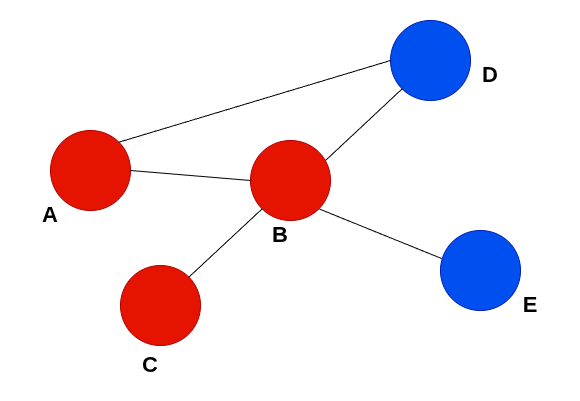
\includegraphics[width=.7\linewidth]{pictures/same_partition_example}
		\caption{Partitioned graph with a volume of 4, each partition has an outgoing volume of 2.}
		\label{3}
	\end{minipage}\qquad
	\begin{minipage}[t]{.4\textwidth}
		\centering
		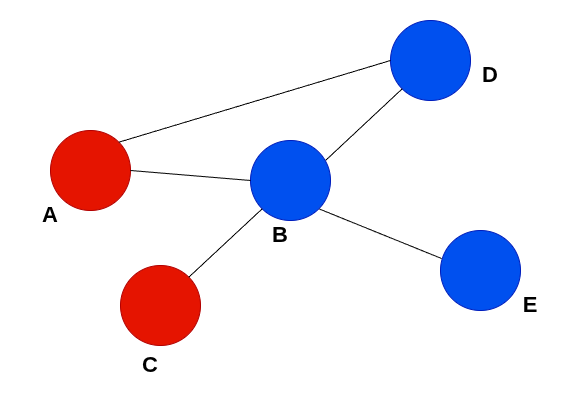
\includegraphics[width=.7\linewidth]{pictures/same_partition_example_moved}
		\caption{Partitinoed graph with a volume of 4, each partition has an outgoing volume of 2 after the move.}
		\label{4}
	\end{minipage}
\end{figure}

Vertex \textit{A} has one edge to the blue partition and contributes $1$ to the communication volume. Vertex \textit{B} has two edges incident to the blue partition, but contributes only $1$ under the given definition. Similarly, vertices \textit{D} and \textit{E} each contribute $1$. In contrast, vertex \textit{C} contributes nothing, as all its incident edges are internal to its partition.
	
Now consider moving vertex \textit{B} from the red partition to the blue partition, as shown in Figure~\ref{4}. We calculate the gain using the global strategy (Section~\ref{METIS gain calculation}). Let \textit{B} be the candidate vertex with neighbors $\{A, C, D, E\}$. Since there are two partitions, the gain vector $G_B$ has size two. In practice, however, $G_B$ effectively has size one, since $G_B[\text{red}]$ is always zero: a vertex moving from its source partition to the source partition is equivalent to no move at all.

\paragraph{Vertex \textit{A}.}
Vertices \textit{A} and \textit{B} are in the same partition and both already have connections to the blue partition. Hence, the set $N_{B-A}$ is empty and no gain contribution arises.

\paragraph{Vertex \textit{C}.}
Vertex \textit{C} lies in the red partition and has no edges to the blue partition. After moving \textit{B}, \textit{C} gains an inter-partition edge, increasing the communication volume. As shown in \hyperlink{METIS_case_1}{Case 1}, this yields a negative gain:
\[
G_B[\text{blue}] \mathrel{-}= 1.
\]
\paragraph{Vertex \textit{D}.}
Vertex \textit{D} is in the blue partition meaning that a move to the blue partition would decrease its volume only if one edge were incident on the red partition. Since \textit{D} has two, \hyperlink{METIS_case_3}{Case 3} does not apply, moving \textit{B} does not change its contribution, hence no case applies.

\paragraph{Vertex \textit{E}.}
Vertex \textit{E} satisfies \hyperlink{METIS_case_2}{Case 2}: it has exactly one connection to the red partition. After the move, this connection disappears, reducing the communication volume and yielding a positive gain:
\[
G_B[\text{blue}] \mathrel{+}= 1.
\]

\hyperlink{METIS_case_4}{Case 4} does not apply, as \textit{B} has multiple connections within its original partition. Summing all contributions yields total gain $0$, so the communication volume remains unchanged.

\paragraph{NVOL gain formulation.}
Using the formulation from Section~\ref{Partition specific gain calculation}, we obtain the same result. We use the table $SG_B$ with size $2\times 1$ (the source column will always be zeroed out just like the source in the gain vector), to store each volume change. As shown above only vertices \textit{C} and \textit{E} contribute:
\[
SG_B[\text{red}][\text{blue}] \mathrel{-}= 1, \quad
SG_B[\text{blue}][\text{blue}] \mathrel{+}= 1.
\]
Additionally, accounting for the direct effect of moving \textit{B} via Equations~\ref{eq:source_global_gain} and~\ref{eq:destination_global_gain}:
\[
SG_B[\text{red}][\text{blue}] \mathrel{+}= 1, \quad
SG_B[\text{blue}][\text{blue}] \mathrel{-}= 1.
\]
The net effect is zero, confirming that neither total nor per-partition volume changes.
\subsection{Three partition example}
We now extend the example to three partitions. Consider the graph in Figure~\ref{three_partition_one_each}, where all vertices have unit weight. The partitions are: red $\{A,B\}$, blue $\{C,D\}$, and green $\{E\}$. The total communication volume is $8$, with partition volumes $3$, $3$, and $2$, respectively.
\begin{figure}[H]
	\centering
	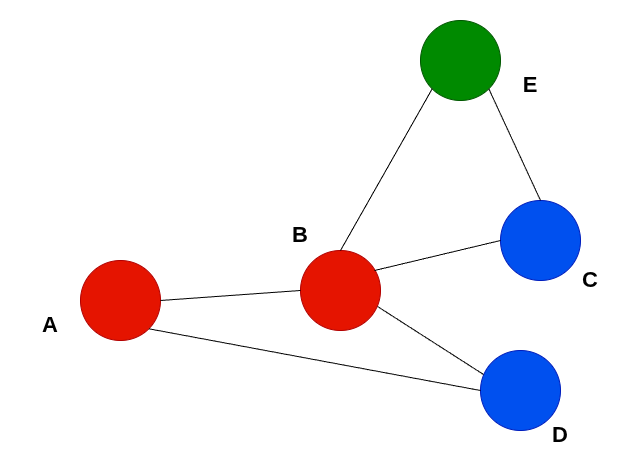
\includegraphics[width=.35\linewidth]{pictures/three_partition_one_each}
	\caption{Partitioned graph with a total communication volume of 8.}
	\label{three_partition_one_each}
\end{figure}
Let \textit{B} be the candidate vertex with neighbors $\{A,C,D,E\}$. Unlike the previous example, \textit{B} may move to either the blue or green partition. Thus, $G_B$ has size 3 and $SG_B$ $3\times 2$.

\paragraph{Vertex \textit{A}.}
Vertex \textit{A} is in the same partition as \textit{B}. Since \textit{A} is connected to the blue partition but not the green partition, \hyperlink{METIS_case_1}{Case 1} applies only for a move to green, introducing a new inter-partition edge:
\[
G_B[\text{green}] \mathrel{-}= 1.
\]

\paragraph{Vertex \textit{C}.}
Vertex \textit{C} is outside the red partition and has exactly one edge to it. By \hyperlink{METIS_case_2}{Case 2}, removing this edge reduces the communication volume. Since \textit{C} is connected to both the blue and green partitions:
\[
G_B[\text{blue}] \mathrel{+}= 1, \quad
G_B[\text{green}] \mathrel{+}= 1.
\]

\paragraph{Vertex \textit{D}.} Vertex \textit{D} has two edges to the red partition. By \hyperlink{METIS_case_3}{Case 3}, a gain change occurs only when the destination partition is not already adjacent to \textit{D}. This holds for the green partition:
\[
G_B[\text{green}] \mathrel{-}= 1.
\]

\paragraph{Vertex \textit{E}.} Vertex \textit{E} is symmetrical to \textit{C}, yielding:
\[
G_B[\text{blue}] \mathrel{+}= 1, \quad
G_B[\text{green}] \mathrel{+}= 1.
\]

Summing contributions gives:
\[
G_B = [0, 2, 0],
\]
indicating that moving \textit{B} to the blue partition reduces the total communication volume by $2$, while moving it to the green partition leaves it unchanged. 

\paragraph{NVOL gain formulation.}
The vector $G_B$ alone does not capture how the volume is redistributed among individual partitions. Using Section~\ref{Partition specific gain calculation}, we compute $SG_B$ as follows.

\paragraph{Vertex \textit{A}.} Vertex \textit{A} follows \hyperlink{NVOL_case_1}{Case 1}for a move to the green partition, yielding:
\[
SG_B[\text{red}][\text{green}] \mathrel{-}= 1
\]

\paragraph{Vertex \textit{C}.} Vertex \textit{C} follows \hyperlink{NVOL_case_2}{Case 2} for both moves, yielding:
\begin{align*}
	SG_B[\text{blue}][\text{blue}] \mathrel{+}= 1 \\
	SG_B[\text{blue}][\text{green}] \mathrel{+}= 1
\end{align*}

\paragraph{Vertex \textit{D}.} Vertex \textit{D} falls under \hyperlink{NVOL_case_3}{Case 3} for the green partition, yielding: 
\[
SG_B[\text{blue}][\text{green}] \mathrel{-}= 1,
\]

\paragraph{Vertex \textit{E}.} Vertex \textit{E} is symmetrical to \textit{C}, yielding:
\begin{align*}
	SG_B[\text{green}][\text{blue}] \mathrel{+}= 1 \\
	SG_B[\text{green}][\text{green}] \mathrel{+}= 1
\end{align*}
Additionally, accounting for the direct effect of moving \textit{B} via Equations~\ref{eq:source_global_gain} and~\ref{eq:destination_global_gain}:
\[
SG_B[\text{red}][\text{blue}] \mathrel{+}= 2, \quad
SG_B[\text{red}][\text{green}] \mathrel{+}= 2,
\]
\[
SG_B[\text{blue}][\text{blue}] \mathrel{-}= 2, \quad
SG_B[\text{green}][\text{green}] \mathrel{-}= 2.
\]
The resulting table $SG_B$ is:
\[
\begin{blockarray}{ccc}
	& \text{blue} & \text{green} \\
	\begin{block}{c(cc)}
		\text{red}   & 2 & 1 \\
		\text{blue}  & -1 & 0 \\
		\text{green} & 1 & -1 \\
	\end{block}
\end{blockarray}
\]

Each column corresponds to a destination partition, and each row describes how a partition's volume changes. One can verify that the column sums recover $G_B$: the sums are 0 (the red partition is implied as no move occurs if the vertex stays in the same partition it already part of), $2+(-1)+1=2$ and $1+0+(-1)=0$ , consistent with $G_B = [0,2,0]$. This formulation provides finer insight: although moving \textit{B} to the green partition leaves the total volume unchanged, it redistributes volume across partitions. In particular, the blue partition experiences an increase in volume at the partition level.

\begin{figure}[H]
	\centering
	\begin{minipage}[t]{.4\textwidth}
		\centering
		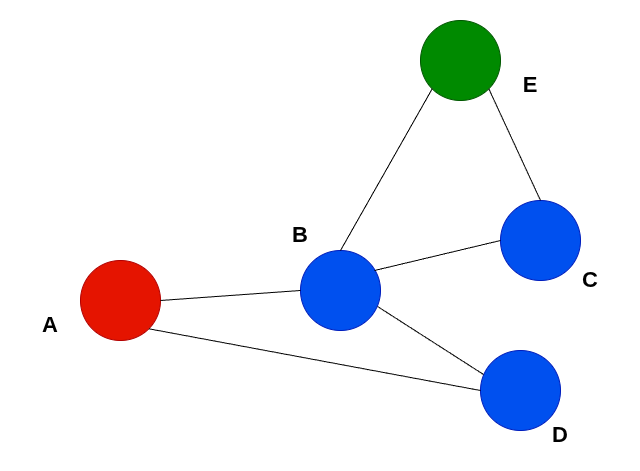
\includegraphics[width=.7\linewidth]{pictures/three_partition_one_each_moved_blue}
		\caption{Partitioned graph has a volume of 6 after \textit{B} is moved to the blue partition}
		\label{three_partition_one_each_moved_blue}
	\end{minipage} \qquad
	\begin{minipage}[t]{.4\textwidth}
		\centering
		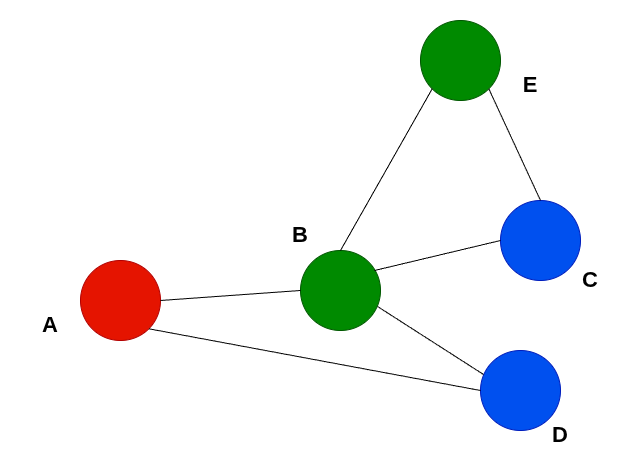
\includegraphics[width=.7\linewidth]{pictures/three_partition_one_each_moved_green}
		\caption{Partitioned graph has a volume of 8 after \textit{B} is moved to the green partition}
		\label{three_partition_one_each_moved_green}
	\end{minipage}
\end{figure}
\subsection{Case 4 example}
None of the preceding examples illustrate a scenario in which Case 4 is relevant. To clarify how such a case may arise and how it affects the communication volume, consider Figure~\ref{case4_example}, where all vertices carry unit weight. The partition assignment is as follows: red $\{A,B,C,G\}$, blue $\{D,E\}$, and green $\{F\}$. The total communication volume is $8$, with individual partition volumes of $3$, $3$, and $2$, respectively. As in the previous example, let $G_C$ have size 3 and $SG_C$  size $3\times 3$.

\begin{figure}[H]
	\centering
	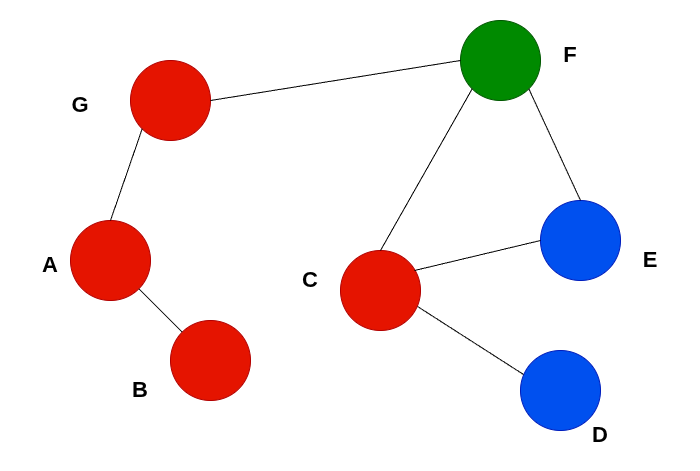
\includegraphics[width=.35\linewidth]{pictures/case4_example}
	\caption{Partitioned graph with a total communication volume of 8.}
	\label{case4_example}
\end{figure}

The candidate vertex is $C$, which has no internal edges within the red partition. Despite the graph containing additional vertices, only the direct neighbors $\{D, E, F\}$ of $C$ need to be visited in order to compute the gain. This illustrates how, even in large graphs, gain computation remains local to the immediate neighborhood of the moving vertex. For conciseness, both computation strategies are consolidated in this example, as they have been thoroughly demonstrated in earlier sections.

\paragraph{Vertex \textit{D}.} Vertex \textit{D} satisfies Case 2 for a move to the blue partition, yielding:
\begin{align*}
	G_C[\text{blue}]\mathrel{+}= 1 \\
	SG_C[\text{blue}][\text{blue}] \mathrel{+}= 1
\end{align*}

\paragraph{Vertex \textit{E}.} Vertex \textit{E} satisfies Case 2 for all possible moves of \textit{C}, yielding: 
\begin{align*}
	G_C[\text{blue}]\mathrel{+}= 1 \\
	G_C[\text{green}]\mathrel{+}= 1 \\
	SG_C[\text{blue}][\text{blue}] \mathrel{+}= 1 \\
	SG_C[\text{blue}][\text{green}] \mathrel{+}= 1
\end{align*}

\paragraph{Vertex \textit{F}.} Vertex $F$ has two edges connecting it to the red partition; however, the set $N_{C-F}$ is empty, meaning Case 3 does not apply and vertex $F$ contributes no change to the gain

\paragraph{Case 4.} Since vertex $C$ has no internal edges, any move will reduce the volume of its source partition. Under normal circumstances, when the candidate vertex has at least one internal edge, moving it leaves the receiving partition's incoming volume unchanged through the candidate. In this case, however, it is necessary to increment the gain for every possible destination partition, yielding:
\begin{align*}
 	G_C[\text{blue}]\mathrel{+}= 1 \\
 	G_C[\text{green}]\mathrel{+}= 1 \\
 	SG_C[\text{blue}][\text{blue}] \mathrel{+}= 1 \\
 	SG_C[\text{green}][\text{green}] \mathrel{+}= 1
\end{align*}
The resulting vector $G_C = [0\,3\,2]$. Accounting for the direct effect of relocating $C$ via Equations~\ref{eq:source_global_gain} and~\ref{eq:destination_global_gain}:
\[
SG_C[\text{red}][\text{blue}] \mathrel{+}= 2, \quad
SG_C[\text{red}][\text{green}] \mathrel{+}= 2,
\]
\[
SG_C[\text{blue}][\text{blue}] \mathrel{-}= 2, \quad
SG_C[\text{green}][\text{green}] \mathrel{-}= 2.
\]
The resulting table $SG_C$ is:
\[
\begin{blockarray}{ccc}
	& \text{blue} & \text{green} \\
	\begin{block}{c(cc)}
		\text{red}   & 2 & 2 \\
		\text{blue}  & 1 & 1 \\
		\text{green} & 0 & -1 \\
	\end{block}
\end{blockarray}
\]
Figures~\ref{case4_example_moved_blue} and~\ref{case4_example_moved_green} show the resulting graphs after moving \textit{C} to the blue and green partitions respectively. The reader can verify that the partition volumes in each case are consistent with the gains predicted by $SG_C$ and $G_C$. Without accounting for Case 4, the gain calculation would be incomplete, potentially leading to incorrect volume estimates when a vertex has no internal edges.
\begin{figure}[H]
	\centering
	\begin{minipage}[t]{.4\textwidth}
			\centering
			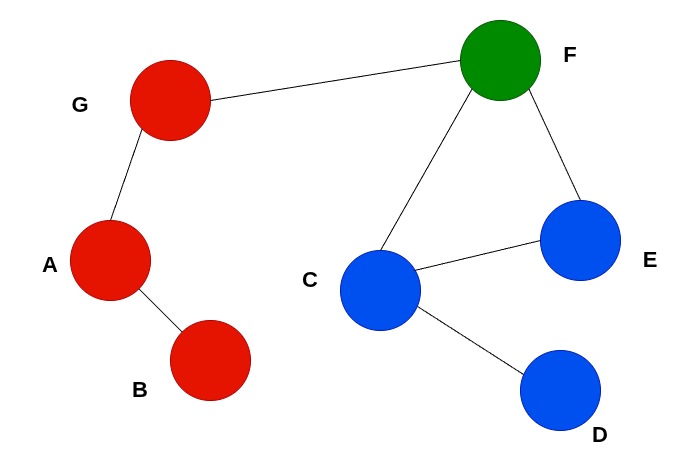
\includegraphics[width=.7\linewidth]{pictures/case4_example_moved_blue}
			\caption{Partitioned graph has a volume of 5 after the move.}
			\label{case4_example_moved_blue}
		\end{minipage}\qquad
	\begin{minipage}[t]{.4\textwidth}
			\centering
			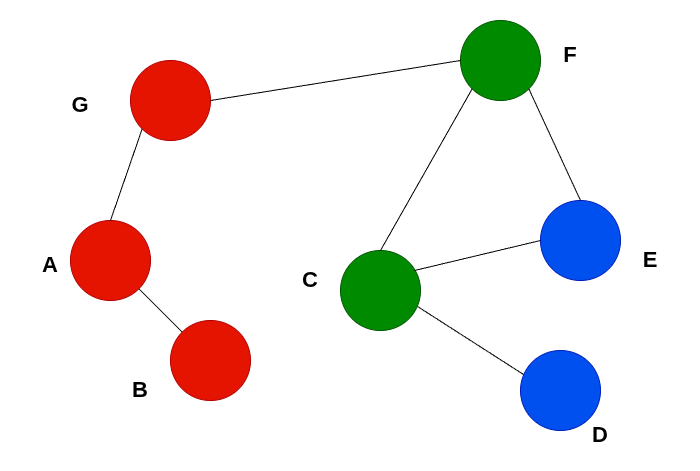
\includegraphics[width=.7\linewidth]{pictures/case4_example_moved_green}
			\caption{Partitioned graph has a volume of 6 after the move.}
			\label{case4_example_moved_green}
		\end{minipage}
\end{figure}

%\section{Implementation}
%%\label{cv_calc_implementation}
%We now describe how the calculation of communication volume change is integrated into the multilevel framework. As mentioned previously, we have used METIS as the base on which to develop NVOL. The following description bridges the formal definitions above and the implemented code.
%
%\subsection{NVOL gain implementation} \label{sec:partition specific gain imp}